\documentclass[letterpaper, 10 pt, conference]{ieeeconf}  

\IEEEoverridecommandlockouts                             
\overrideIEEEmargins

\usepackage{graphics} 
\usepackage{graphicx}
\usepackage{epsfig} 
\usepackage{mathptmx} 
\usepackage{times} 
\usepackage{amsmath} 
\usepackage{amssymb}  
\usepackage{makeidx}
\usepackage{float}
\usepackage{balance}
\usepackage{url}
\usepackage{hyperref}
\usepackage{cite}
\usepackage{flexisym}
\usepackage{chngcntr}
\usepackage{tikz}

\newtheorem{assumption}{\textbf{Assumption}}
\newtheorem{definition}{\textbf{Definition}}


\DeclareMathOperator*{\maxi}{max}
\DeclareMathOperator*{\mini}{min}

\title{\LARGE \bf Integrated Online Perception of Articulated Objects for Manipulation}

\author{Jia Guo \and George Kontoudis
\thanks{J. Guo and G. Kontoudis are with the Mechanical Engineering Department, Virginia Polytechnic Institute and State University, Blacksburg, VA, 24060, USA.}% Stops a space
\thanks{Names were alphabetically ordered.}}

\begin{document}
\maketitle
\thispagestyle{empty}
\pagestyle{empty}

\begin{abstract}
An online interactive perception methodology for articulated objects in unstructured environment is presented. The main contribution of this methodology lies in the online solution, which utilize recursive Bayesian estimation techniques. The RGB-D algorithm consist of three sub-recursive estimation problems and each one forms a separate level of estimation. In this way, we can get uncomplicated solution at each level which feed forward and backward information to guarantee robustness, accuracy, and uncertainty elimination. The efficacy of the proposed method is verified through robot manipulation experiments.     
\end{abstract}

\normalsize{\bf\small\emph{Index Terms:} Online perception, recursive Bayesian estimation, manipulation}  

\section{Introduction}\label{intro}
An online mutli-level interactive perception algorithm is presented \cite{martin2014online}, \cite{martin2016integrated}. Grasping and manipulation in unstructured environments require knowledge of the object's shape, position, orientation, and kinematic structure. Visual perception could be a solution to successfully get the information needed for robotic manipulation. Although, it becomes non-trivial to online address this problem and estimate robust solutions. However, the allocation to sub-level algorithms which are interconnected, simplify the overall solution.

In this project we deal with online interactive perception algorithm for robotic manipulation purposes. The algorithm includes the identification of the object's shape, the recognition of its kinematic structure, and the motion tracking of its position and orientation. Moreover, the derivation of the explored object's shape, position, orientation, along with the kinematic structure is achieved. The object's position, orientation, and estimation of kinematic structure part incorporates three recursive Bayesian estimation steps. Then, the shape reconstruction of the investigated object is addressed that thrust the motion tracking.

Robotic manipulation is an emerging field for many decades. \cite{chang2012interactive}, \cite{sturm2010vision}, \cite{katz2014interactive}, \cite{thrun2005probabilistic}, \cite{tomasi1991detection}, \cite{brock2009learning}, \cite{krainin2011manipulator}, \cite{wuthrich2013probabilistic}, \cite{choi2013rgb}, \cite{mishra2009active}, \cite{yuheng2013star3d}, \cite{herbst2014toward}, \cite{pomerleau2011tracking}.

The remainder of this report is organized as follows. Section \ref{pf} discusses the problem formulation. %Algorithm representation is provided in section \ref{algAn}. 
The efficacy of the proposed methodology is assessed in Section \ref{experim} by a set of experiments. Section \ref{resul} discusses the results of this project. Finally, Section \ref{concl} provides the conclusions of the studied methodology and gives directions for future work.  

% Then, object's motion segmentation is performed to identify motion variations.

\section{Problem Formaulation}\label{pf}
In this section we formulate the proposed methodology for integrated online perception. First, the interactive perception problem tracks the motion, and estimates the kinematic structure of the object. Then, this information is provided to the tracker which performs feautre-based tracking, and shape based tracking along with information given from shape-based reconstruction module. The motion segmentation in color and in depth follows to identify fault information from the environment. Next, the object's reconstruction takes place by separating the unreliable information from the picture. Finally, shape-based segmentation is accomplished to feed the shape-based tracking. In figure \ref{RE} the kinematic structure of the methodology is depicted. 

\begin{figure}[!h]
	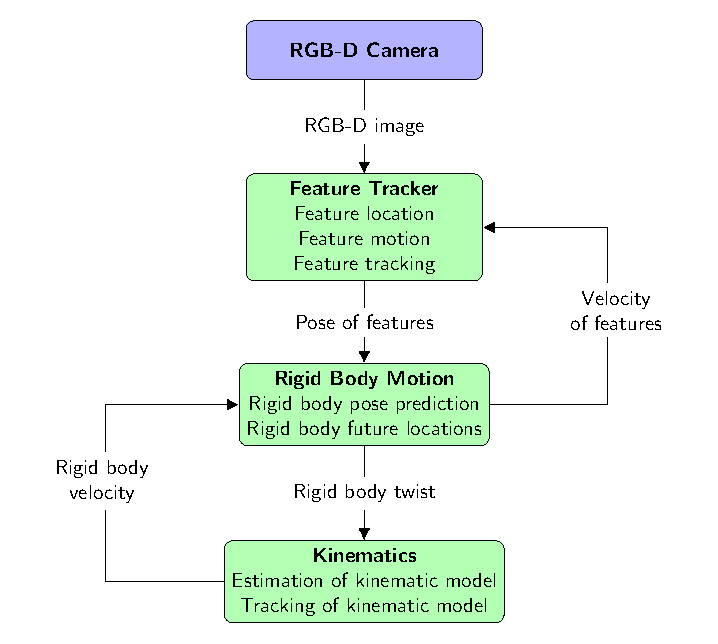
\includegraphics[scale=0.70]{figures/RecursiveEstimation.pdf}
	\centering
	\caption{Kinematic identification scheme.}
	\label{RE}
\end{figure}

\subsection{Feature Motion Estimation}\label{fme}
The gathered information from an RGB-D camera employed to track feature motion with recursive estimation. The recursive estimation seeks to update the belief of target $p(x_k^t|z_{1:k}^t)$. In this case the targets are features of the object in the $3D$ space, $x_k^f \in \mathbb{R}^{3m}$, where $k \in \mathbb{N}$ is the time index, $f$ is the feature motion, and $m \in \mathbb{N}$ is the number of features we track. Then we get observations from the camera in the 2-$D$ image plane, $z_k^f \in \mathbb{R}^{2m}$, where $k \in \mathbb{N}$ is the time index, $f$ is the feature motion, and $m \in \mathbb{N}$ is the number of features we track. 

The recursive estimation is based on priors of Kanade-Lucas-Tomasi (KLT) tracking algorithm \cite{tomasi1991detection}, \cite{lucas1981iterative} the small motion, and the brightness constancy constraint. Small motion means that the feature points do not move far away from their previous position. Brightness constancy means that the projection of the same feature is the same at each frame. 
%The brightness constancy equation yields
%\begin{equation}
%I(x,y,t)=I(x+u,y+v,t+1)
%\end{equation}
First, a feature initialization takes place from the image, based on Kanade-Tomasi corner detection. Then, a prediction of 3-$D$ feature's location is occurred from its current location and the velocities obtained from the higher stage. Next, this prediction is employed to project this features in the image plane and use them as input to KLT algorithm. 

\subsection{Extended Kalman Filter of Rigid Bodies}\label{EKFrb}
In the second stage an extended Kalman filter (EKF) is utilized to estimate the motion of rigid bodies. The information needed is collected form the lower stage feature tracker and from the upper stage kinematic model estimator. The methodology deals with EKF, because it is based on non-linear Gaussian models. The stochastic motion and sensor models have the form of
\begin{equation}
x_k^t=f^t(x_{k-1}^t,u_{k-1}^t)+w_{k-1}^t,
\end{equation} 
\begin{equation}\label{obsM}
z_{k-1}^t=h^t(x_{k-1}^t)+v_{k-1}^t,
\end{equation} 
where $k \in \mathbb{N}$ is the time index, $x_k^t$ is the vector of states, $z_{k-1}^t$ is the vector of observations, $w_{k-1}$ and $v_{k-1}$ are the zero-mean independent identically distributed Gaussian noises $w_{k-1}^t \sim \mathcal{N}(0, \Sigma_{w_{k-1}^t})=\mathcal{N}(0, Q_{k-1})$, with $Q_{k-1} \geq 0$, and $v_{k}^t \sim \mathcal{N}(0, \Sigma_{v_{k-1}^t})=\mathcal{N}(0, R_{k-1})$ with $R_{k-1}>0$.
To estimate the state, the EKF first predicts the state and the covariance as
\begin{equation}
\bar{x}_{k|k-1}^t=f^t(x^t_{k-1|k-1},u^t_{k-1}),
\end{equation}
\begin{equation}
\Sigma_{x_{k|k-1}^t}=A_{k-1} \Sigma_{x_{k-1|k-1}^t} A_{k-1}^{\intercal} +Q_{k-1},
\end{equation}
where
\begin{equation}
A_{k-1}= \frac{\partial f^t(x_{k-1|k-1}^t,u_{k-1})}{\partial x_{k-1|k-1}^t}.
\end{equation}
Then the Kalman gain is calculated from 
\begin{equation}
K_{k}= \Sigma_{x_{k|k-1}^t} C_k^{\intercal}(C_k \Sigma_{x_{k|k-1}^t} C_k^{\intercal}+ R_{k})^{-1},
\end{equation}
where
\begin{equation}
C_k= \frac{\partial h^t(x_{k|k-1}^t)}{\partial x^t_{k|k-1}}.
\end{equation}
Next, the correction is given as
\begin{equation}
\bar{x}_{k|k}^t=\bar{x}_{k|k-1}^t+K_k(z_k^t-h^t(\bar{x}_{k|k-1})),
\end{equation}
\begin{equation}
\Sigma_{x_{k|k}^t}=(I-K_kC_k)\Sigma_{x_{k|k-1}^t}.
\end{equation}

More specifically the correct features from the lower stage are defined as rigid bodies. Every rigid body has its own EKF and the state composed from position and orientation, and twist, $x_k^t = [ p^{\intercal} \hspace{.2cm} \nu^{\intercal} ] ^{\intercal}$, $x_k^t \in \mathbb{R}^{12}$. The observations contain the location of each rigid body in the 3-$D$ space, $z_k^t \in \mathbb{R}^{3m}$. Three simultaneous actions were employed to predict the state of rigid bodies. One action predicts the next state of rigid bodies by employing an EKF as previously described. The other action examines the sudden immobilization of rigid bodies, while the last action employs data from the upper kinematic stage to predict an alternative state of rigid bodies. The observation part includes feature locations in 3-$D$ space $f_0^m$ and the homogeneous transformation using the position and orientation of the rigid bodies $T(p)$. The exact probabilistic sensor model of \ref{obsM} becomes
\begin{equation}\label{obsMF}
z_k^t=h^t(x_{k-1}^t)+v_{k-1}^t= \begin{bmatrix}
T(p)f^1_{0} \\
\vdots \\
T(p)f^m_{0}
\end{bmatrix} + v_{k-1}^t,
\end{equation}

To effectively estimate the motion of a group with multiple rigid bodies the generation of valid sets is needed. After defining these sets the next step is to estimate their motion in 3-$D$ space. For this purpose we employ EKF to predict the group motion, but in case that the error exceeds $2cm$, random sample consensus (RANSAC) is utilized. If the group consists of at least $15$ features we consider it as a valid set.



\subsection{Extended Kalman Filter of Kinematic Model}\label{EKFkm}
An estimation and tracking of the kinematic model is achieved in the third stage. The information needed is gathered from the lower stage rigid body estimator. The kinematic model can be related either as a prismatic joint, or as a revolute joint, or as a rigid connection, or unrelated. Each relation is represented by a different state $x_{joint}^t$ and the observations are collected form the previous stage as a set of multiple rigid bodies $z_{joint}^t \in \mathbb{R}^6$, along with the zero-mean independent identical distributed Gaussian noise $v_{joint}^t$. Since, the type of joint varies the utilization of different observation model was imposed to apply EKF. 

For the prismatic joint estimation the state includes the axis orientation, the joint displacement $q_p \in \mathbb{R}$, and the joint velocity. Joint velocities update by employing the previous stage twist vector. For the position and orientation prediction of the rigid bodies relation, the following observation model was utilized
\begin{equation}
z_{pr, joint}^t=\begin{bmatrix}
q_p \hat{o}_p\\
0_3 
\end{bmatrix} + v_{k-1}^t,
\end{equation}
where $\hat{o}_p \in \mathbb{R}^3$ is the orientation of the axis.

For the revolute joint estimation the state includes the axis orientation, the joint revolution $q_r \in \mathbb{R}$, and the joint velocity. Joint velocities update by employing the previous stage twist vector. For the position and orientation prediction of the rigid bodies relation, the following observation model was utilized
\begin{equation}
z_{rev, joint}^t=\begin{bmatrix}
(-q_r \hat{o}_r) \times p_r\\
q_r \hat{o}_r
\end{bmatrix} + v_{k-1}^t,
\end{equation}
where $\hat{o}_p \in \mathbb{R}^3$ is the orientation of the axis, and $p_r \in \mathbb{R}^3$ is a point on the axis of rotation.

The observation for rigid boy estimation has no information about rigid body relations $z_{rig, joint}^t = 0_6 + v_{k-1}^t$. In case none of the above stands then the algorithm defines unrelated rigid bodies.













%\section{Algorithm Analysis}\label{algAn}

\section{Experiments}\label{experim}

\section{Results}\label{resul}

\section{Conclusions}\label{concl}

\bibliographystyle{IEEEtrans}
\bibliography{IEEEabrv,mybib}

\end{document}